\documentclass[a4paper,12pt,oneside]{memoir}
%Pacotes
\usepackage[english,brazil]{babel}%Idioma
\usepackage[utf8]{inputenc}%Inserir acentos 
\usepackage[T1]{fontenc}%Tipo de fonte usada na compilação
\usepackage{hyphenat}%Habilita/desabilita hifenização
%Ativar se necessário
%\setlength{\parskip}{1\baselineskip}%Espaçamento de 1pt entre os parágrafos
\usepackage{setspace}%Mudar espaçamento entre linhas
\usepackage[a4paper,%
            left=3.0cm,%
            right=2.0cm,%
            top=3.0cm,%
            bottom=2.0cm]{geometry}
\usepackage{graphicx}%inserir imagens
\usepackage[x11names]{xcolor}%Texto colorido
\usepackage{pdfpages}%Inserir páginas PDF
\usepackage{multicol}%Criar multicolunas sem \tabular
\usepackage{xurl}%Para disponibilizar o endereço do site
\usepackage[breaklinks,hidelinks,colorlinks=true,allcolors=blue]{hyperref}%Configurar hiperlinks
\usepackage{tabularx}%Tabelas mais fáceis
\usepackage{booktabs}
\usepackage{textcmds}%Digitar aspas com \qq e \q
\usepackage{lipsum}%Gerar Lipsum
\usepackage{indentfirst}%Indentar 1º§ de cada seção
\usepackage{microtype}%Melhorar a justificação do texto


%Referências e Citações
\usepackage[alf,
            abnt-emphasize=bf,%
            abnt-etal-list=3,%
            abnt-etal-text=emph,%
            abnt-missing-year=sd,%
            abnt-repeated-author-omit=yes,%
            abnt-repeated-title-omit=yes,%
            abnt-thesis-year=final,%
            abnt-doi=link,%
            ]{abntex2cite}

%Comandos e Ambientes
%Autor
\newcommand{\me}{\begin{center}{André Alexandre Padilha Leitão}\end{center}}

%Resumo
\renewenvironment{abstract}
  {\small\quotation
  {\bfseries\noindent{\normalsize\abstractname}\par\nobreak\smallskip}}
  {\endquotation}

%Citação +3 linhas
\usepackage{changepage}
\newenvironment{citar}
{\begin{adjustwidth}{4cm}{0cm}\SingleSpacing\footnotesize\par}
{\end{adjustwidth}}

%Texto da folha de rosto (tipo de trabalho)
\newenvironment{textofolharosto}
{\SingleSpacing\small\list{}{\rightmargin=0cm \leftmargin=7cm}%
	\item\relax}%
{\endlist}

%Definições dos capítulos
\chapterstyle{section}%Título somente com o número e o nome, sem "Capítulo X" da classe
\pagestyle{simple}
\aliaspagestyle{part}{empty}
\setsecnumdepth{subsubsection}

%Caixa de texto para uso com códigos
\usepackage{tcolorbox}
\tcbuselibrary{most,listingsutf8}% 
\newtcblisting[auto counter,number within=chapter]{codex}[2][]{%
	arc=0mm,
	listing only,
	colback=black!5!white,
	colframe=black!75!white,
	fonttitle=\bfseries,
	title=Exemplo \thetcbcounter: #1 #2,
	listing options={style=tcblatex,numbersep=1mm,numbers=left,numberstyle=\tiny\color{black}}
}
%Início pré-textuais (capa, folha de rosto e sumário)
\begin{document}
\frontmatter{
    \begin{titlingpage}
    %PREENCHA OS CAMPOS ABAIXO COM AS INFORMAÇÕES DO SEU TRABALHO
\author{Nome completo do autor}
\title{Título do projeto}
%Data da defesa. Apenas mês e ano.
%Mude o mês para informar a data de apresentação do PROJETO
\date{Jan. \the\year{}{}}

%INFORMAÇÕES DA INSTITUIÇÃO, CURSO E ORIENTADOR
\newcommand{\instituicao}{Instituto Federal de Pernambuco}
\newcommand{\campus}{Campus Garanhuns}
\newcommand{\localdefesa}{Garanhuns - PE}
\newcommand{\curso}{Tecnólogo em Análise e Desenvolvimento de Sistemas}
\newcommand{\orientador}[1]{\textbf{Orientador/a:} #1}

%FORMATAÇÃO DO ELEMENTOS PRÉ-TEXTUAIS - NÃO ALTERAR
%Capa
\begin{center}
%CAPA
%CASO NÃO DESEJE O LOGO DA INSTITUIÇÃO, EXCLUIR LINHA ABAIXO.

\includegraphics[scale=.10]{./img/logo-ifpe.png}\\
\textbf{\textsc{\instituicao}}\\
%Caso sua instituição não tenha CAMPUS, remova o comando \campus.
\textbf{\textsc{\campus}}\\

\vspace*{5cm}
\textbf{\thetitle}\\
\textbf{\theauthor}

\vspace*{\fill}
\localdefesa\\
\thedate
\end{center}

%FOLHA DE ROSTO + TIPO DE TRABALHO
\frontmatter{
\newpage
\thispagestyle{empty}
\begin{center}
	\textbf{\theauthor}
	
	\vspace*{5cm}
	\textbf{\thetitle}
\end{center}
%Caso sua instituição não tenha CAMPUS, remova o comando \campus.
%ATENÇÃO À PRESPOSIÇÃO "AO/À"
	\vspace*{2cm}
	\begin{textofolharosto}
	Projeto de trabalho de conclusão de curso apresentado ao \instituicao\ \campus\ como requisito para elaboração do trabalho final do curso de \curso.\\
	\ \\
    \ \\
    \orientador {Nome do orientador}
	\end{textofolharosto}

\begin{center}
\vspace*{\fill}
\localdefesa\\
\thedate
\end{center}

%RESUMO e ABSTRACT
%Ler instruções em resumo+abstract.tex
%\input{pretxt/resumo+abstract.tex}


    \end{titlingpage}
%Sumário, lista de figuras, lista de tabelas.
\tableofcontents*
\thispagestyle{empty}
\newpage\listoffigures*
\thispagestyle{empty}
\newpage\listoftables*
\thispagestyle{empty}
}
%Fim pré-textuais (capa, folha de rosto e sumário)
%===================================
\savepagenumber
\mainmatter
\restorepagenumber
\pagestyle{simple}
\OnehalfSpacing

%Início do texto
\chapter*{Apresentação}
\addcontentsline{toc}{chapter}{Apresentação}

Este modelo de \textbf{PROJETO} de trabalho de conclusão de curso (TCC) foi elaborado para os estudantes dos cursos de graduação do Instituto Federal de Pernambuco Campus Garanhuns (IFPE/GUS).

Não se trata de um modelo para trabalho final, isto é, o TCC propriamente dito. Para esse modelo ver \url{https://github.com/TheMemoir}.

Procurei seguir as normas ABNT para elaboração de trabalhos acadêmicos, em especial as NBR 15287:2011 e as demais a elas relacionadas, tais como:

\begin{itemize}
\itemsep0em
    \item ABNT NBR 6023, Informação e documentação – Referências – Elaboração
    \item ABNT NBR 6024, Informação e documentação – Numeração progressiva das seções de um
    documento – Apresentação
    \item ABNT NBR 6027, Informação e documentação – Sumário – Apresentação
    \item ABNT NBR 10520, Informação e documentação – Citações em documentos – Apresentação
    \item IBGE. Normas de apresentação tabular. 3. ed. Rio de Janeiro, 1993
\end{itemize}

Apesar de existir um repositório institucional (RI) no IFPE (ver \url{https://repositorio.ifpe.edu.br/xmlui/}, não há -- no âmbito institucional -- um modelo que se aplique aos trabalhos desenvolvidos na instituição para depósito no RI, seja nos níveis do Ensino Médio, Ensino Subsequente, Ensino Superior ou Ensino de Pós-graduação.

Nesse sentido, o presente modelo serve para que os estudantes possam se familiarizar com o uso do \LaTeX, já que se trata de um projeto a ser apresentado ao orientador para, posteriormente, poder usar o modelo de TCC, também em \LaTeX, disponível no GitHub (ver acima) e possível de ser utilizado no Overleaf\footnote{\url{https://pt.overleaf.com/}}.

A primeira seção deste modelo trata sobre as referências bibliográficas, item essencial para construção cientifica do trabalho e também para citações e a própria seção de referências. Baseia-se na ABNT NBR 6023:2018 e no pacote \verb|abntex2cite|\footnote{\url{http://tug.ctan.org/macros/latex/contrib/abntex2/doc/abntex2cite.pdf}}.

A segunda seção trata das citações no texto que, devem somente ser feitas após construção das referências bibliográficas (ou no máximo ao mesmo tempo...). Baseia-se na norma ABNT NBR 10520:2002 e, também no pacote \verb|abntex2cite|.

A terceira seção trata da inserção de tabelas e figuras no \LaTeX com referências cruzadas e geração automática na parte pré-textuais \textbf{Listas}.

A quarta seção exemplifica o uso de alguns ambientes específicos criados para este modelo que também podem ser usado no modelo de trabalho final\footnote{endereço no GitHub}, como também dos elementos pós-textuais opcionais Anexos e Apêndices.

Espero que seja útil.

\begin{flushright}
André Padilha

Março de 2023
\end{flushright}

%===================================
\chapter{Referências}
As referências no \LaTeX são construídas em um arquivo separado com extensão \verb|.bib|. Neste modelo, o arquivo chama-se \verb|references.bib| e já contém boa parte de exemplos dos tipos de referências mais utilizados: livros, capítulos de livro, artigos, manuais, dissertações e teses.

Não é necessário apagar as entradas já existentes. Basta copiá-las, substituir as informações conforme a nova entrada bibliográfica e, posteriormente, citar a nova entrada no texto. Veja os exemplos a seguir.
\ \\
\begin{figure}[h!]
\begin{codex}{Livro com um ou mais autores sem (Org.)}
@book{eagleton2011,
	author     = {Terry Eagleton},
	title      = {A ideia de cultura},
	edition    = {2},
	address   = {São Paulo},
	publisher  = {Editora UNESP},
	year       = {2011},
	translator = {Sandra Castello Branco},
}
\end{codex}
\caption{Modelo de entrada bibliográfica - livro}
    \label{fig:codex1}
\end{figure}

Essa entrada bibliográfica produzirá citações de acordo com a NBR ABNT 10520:2002 (ver seção seguinte) e para se utilizar esse modelo, basta copiá-lo e preencher com as informações, conforme a seguir.

\begin{figure}
\begin{codex}{Livro com um ou mais autores sem (Org.) - Modificado}
@book{dosto2013,
	author     = {Fiódor Dostoiévski},
	title      = {O duplo},
	edition    = {},
	address   = {São Paulo},
	publisher  = {Editora 34},
	year       = {2013},
	translator = {Paulo Bezerra},
}
\end{codex}
\caption{Entrada bibliográfica alterada - livro}
    \label{fig:codex2}
\end{figure}

Observe que o início da entrada no exemplo \ref{fig:codex1} é \verb|@book{eagleton2011,|. Isso indica que o material é um livro e que para chamá-lo eu criei a chave \qq{eagleton2011,}. Esse nome quem define é o usuário. Uma boa prática é usar o sobrenome do autor seguido do ano, mas, como dito, pode ser qualquer texto que o usuário deseje. No exemplo \ref{fig:codex2}, a entrada criada por mim foi \verb|@book{dosto2013,|, porque o sobrenome é \q{chato} de escrever (Dostoiévski).

Busquei incluir apenas alguns elementos opcionais para as referências, tais como edição e tradutor (para livro). Caso esses não existam na nova entrada bibliográfica, basta deixar em branco (como em \ref{fig:codex2}) em \verb|edition|.

A mesma lógica segue para os demais tipos de entradas bibliográficas no arquivo \verb|.bib|. Para mais informações sobre referências no \LaTeX com o \verb|abntex2cite|, ver nota de rodapé 2 ou o \textit{site} do projeto em \url{https://www.abntex.net.br/}.

Uma observação que dever ser feita para os arquivos \verb|.bib| que impactam tanto nas citações como na geração das referências é a acentuação. De acordo com o pacote \verb|abntex2cite|, 

\begin{citar}
    Não há problemas em usar caracteres acentuados em arquivos bibliográficos [...] [p]orém, como as regras ABNT exigem a conversão do autor ou organização para maiúsculas, é preciso observar o modo como se escrevem o nome dos autores. \cite[p. 8]{abntex2018}
\end{citar}

%===================================
\chapter{Citações} 

\section{Diretas e Indiretas - Menor que 3 linhas}

Citações podem ser diretas ou indiretas. São citações \textbf{diretas} aquelas que reproduzem \textsc{exatamente} as palavras do autor/a. São incluídas no texto entre aspas duplas (\qq{ }) e o nome do autor citado é mostrado em letras maiúsculas, seguido do ano e, opcionalmente, a página ou páginas. São indiretas aquelas em que você parafraseia, isto é, diz com suas palavras, aquilo que foi dito pelo autor do texto citado. Esse tipo de citação é \qq{mesclado} com o seu texto e mostra o nome do autor citado em minúsculas, seguido do ano e, opcionalmente, a página ou páginas.

Observe os exemplos abaixo.

\begin{enumerate}
\itemsep0em
    \item "As citações diretas, no texto, de até três linhas, devem estar contidas entre aspas duplas. As aspas simples são
utilizadas para indicar citação no interior da citação." \cite{abnt10520}
    \item Conforme a \citeonline[p. 2]{abnt10520}, é possível usar dois tipos de aspas: simples e duplas. As duplas são para citação direta e as simples para citação dentro de uma citação direta. .
\end{enumerate}

O pacote \verb|abntex2cite| permite que, após construída a entrada bibliográfica, se cite utilizando os seguintes comandos:

\begin{enumerate}
    \itemsep0em
    \item \verb|\cite{entrada}|
    \item \verb|\citeonline{entrada}|
    \item \verb|\citeyear{entrada}|
    \item \verb|\citeauthor{entrada}|
\end{enumerate}

Em 1 tem-se a forma de uma citação direta, em que o autor aparece em letras maiúsculas seguido do ano. A chamada é feita desse modo \verb|\cite{fiorin1999}| e o resultado é: \qq{É preciso alertar que o fazer teórico da semiótica é aspectualizado imperfectivamente, o que significa que não constitui ela uma teoria pronta e acabada, mas um projeto, um percurso.} \cite{fiorin1999}.

Observe que se for necessário incluir a página da citação, basta acrescentar no código a página entre colchetes: \verb|\cite[p. 1]{fiorin1999}|. O resultado será: \qq{É preciso alertar que o fazer teórico da semiótica é aspectualizado imperfectivamente, o que significa que não constitui ela uma teoria pronta e acabada, mas um projeto, um percurso.} \cite[p.1]{fiorin1999}.

Em 2 tem-se a forma de uma citação indireta, em que o autor aparece em letras minúsculas, seguido do ano. A chamada é feita desse modo \verb|\cite{eagleton2011}| e o resultado é: Conforme \citeonline{eagleton2011}, a palavra cultura é uma das palavras mais difíceis de nossa língua. Do mesmo modo, havendo necessidade de inclusão da página, o código deve ser feito assim: \verb|\cite[p.1]{eagleton2011}| e o resultado será: Conforme \citeonline[p. 1]{eagleton2011}, a palavra cultura é uma das palavras mais difíceis de nossa língua.

Nos dois casos acima, se existirem mais de um autor que tratem do mesmo tema, basta incluir no código cada entrada separada por vírgulas: \verb|cite{eagleton2011,fiorin1999}| ou \verb|\citeonline{eagleton2011,fiorin1999}| e o resultado será, respectivamente: \cite{eagleton2011,fiorin1999} e \citeonline{eagleton2011,fiorin1999}. 

Já em 3, cita-se apenas o ano da obra e o nome do autor deverá ser informado manualmente, como em: \verb|\citeyear{dionisioetal2005}| cujo resultado será: Em \citeyear{dionisioetal2005} Dionísio trata da multimodalidade nos gêneros textuais... Observe que o ano já aparece com referência cruzada, indicando que a entrada já foi incluída na seção Referências.

Por fim, em 4, tem-se a citação somente do autor, sem indicação do ano ou página. Esses últimos deverão ser feitos manualmente, como em: \verb|\citeauthor{dosto2013}| cujo resultado é: Na obra \textbf{O duplo}, \citeauthor{dosto2013} (2013, p. 190) diz que os inimigos permaneciam calados. Note que esse tipo de citação tanto pode incluir a forma direta ou indireta, já que somente o nome do autor é mencionado no texto.

 \section{Diretas - Maior que 3 linhas}

 Segundo a ABNT 10520,

\begin{citar}
[a]s citações diretas, no texto, com mais de três linhas, devem ser destacadas com recuo de 4 cm da margem esquerda, com letra menor que a do texto utilizado e sem as aspas. \cite[p. 2]{abnt10520}
\end{citar}

O presente modelo de projeto já traz um ambiente específico para esse tipo de citação, o \textbf{citar}. Para a citação acima, da ABNT, o código pode ser visto na figura \ref{fig:codex3}:

\textsc{Importante:} O exemplo de citação que usei acima não reflete o tamanho superior a três linhas. Conta-se o texto/número de linhas até a citação propriamente dita; não se inclui a referência no número de linhas. Trata-se de uma demonstração do comando apenas.
\ \\
\begin{figure}[h!]
\begin{codex}{Ambiente citar e exemplo de citação}
  \begin{citar}
    [a]s citações diretas, no texto, com mais de três linhas, devem ser destacadas com recuo de 4 cm da margem esquerda, com letra menor que a do texto utilizado e sem as aspas. \cite[p. 2]{abnt10520}
  \end{citar}
\end{codex}
\caption{Ambiente \textbf{citar} e exemplo de citação.}
    \label{fig:codex3}
\end{figure}
\ \\
\indent Como se pode ver, inicia-se o ambiente com \verb|\begin{citar}|, inclui-se a citação e finaliza-se com \verb|\end{citar}|. Obviamente, os comandos para referenciar também podem ser usados logo após o texto citado. 

%===================================
\chapter{Tabelas, figuras e referências cruzadas}
Nessa seção, será explicado como referenciar tabelas e figuras de modo que sejam automaticamente criadas as referências cruzadas e, também, a inserção destas referências nas partes pré-textuais a elas destinadas (Lista de Figuras e Lista de Tabelas). Não foi incluída a Lista de Símbolos.

\section{Como criar uma referência cruzada para tabelas}

O exemplo de tabela a seguir tem duas linhas, três colunas, uma legenda com numeração automática e o texto indicativo com uma hiperligação para a tabela que funciona tanto no texto propriamente dito quanto na \textbf{Lista de Tabelas} e \textbf{Lista de Figuras} na parte pré-textual.

\subsection{Tabelas}
\begin{table}[h!]
\begin{center}
\begin{tabularx}{0.8\textwidth} { 
  | >{\centering\arraybackslash}X 
  | >{\centering\arraybackslash}X 
  | >{\centering\arraybackslash}X | }
 \hline
 item 1 & item 2 & item 3 \\
 \hline
 item 4  & item 5  & item 6  \\
\hline
\end{tabularx}
\caption{Tabela de teste 01 para teste de ref. cruzada.}
\label{table:1}
\end{center}
\end{table}

A tabela acima é referenciada por Tabela \ref{table:1}. Note que a numeração da tabela é composta pelo número 3, que indica a seção onde ela se localiza, seguida do número 1, que é a numeração da primeira tabela.

\begin{table}[h!]
\begin{center}
\begin{tabularx}{0.8\textwidth} { 
  | >{\centering\arraybackslash}X 
  | >{\centering\arraybackslash}X 
  | >{\centering\arraybackslash}X | }
 \hline
 item 1 & item 2 & item 3 \\
 \hline
 item 4  & item 5  & item 6  \\
\hline
item 7  & item 8  & item 9  \\
\hline
\end{tabularx}
\caption{Tabela de teste 02 para teste de ref. cruzada.}
\label{table:2}
\end{center}
\end{table}

Já esta tabela é referenciada por tabela \ref{table:2}. O segundo número (2) indica que esta é a tabela número dois.

Para lembrar a \textbf{ordem dos comandos}:

\begin{enumerate}
\itemsep0em
    \item iniciar o ambiente \verb|\begin{table}|
    \item iniciar a centralização \verb|\begin{center}|
    \item iniciar o ambiente tabular \verb|\begin{tabular}|
    \begin{enumerate}
        \item definir a especificação da tabela (linhas, colunas, largura, etc.)
        \item neste caso, a definição depende do ambiente usado para as criação da tabela. Os pacotes \verb|tabularx| e \verb|booktabs| estão incluídos nesse modelo.
        \item aqui foi usado o ambiente \verb|tabularx|
    \end{enumerate}
    \item finalizar o ambiente tabular \verb|\end{tabular}|
    \item finalizar a centralização \verb|\end{center}|
    \item finalizar o ambiente \verb|\end{table}|
    \item definir uma legenda para tabela \verb|\caption{legenda}|
    \item definir uma etiqueta para ref. cruzada \verb|\label{id:tabela}|
\end{enumerate}

Observe o código:
\begin{codex}{Código de exemplo - Tabelas}
\begin{table}[h!]
\begin{center}
\begin{tabularx}{0.8\textwidth} { 
  | >{\centering\arraybackslash}X 
  | >{\centering\arraybackslash}X 
  | >{\centering\arraybackslash}X | }
 \hline
 item 1 & item 2 & item 3 \\
 \hline
 item 4  & item 5  & item 6  \\
 \hline
 item 7  & item 8  & item 9  \\
 \hline
\end{tabularx}
\caption{Tabela de teste 02 para teste de ref. cruzada.}
\label{table:2}
\end{center}
\end{table}
\end{codex}

\textsc{Observação:} Nos códigos de exemplo anteriores existe uma legenda, mas neste último não. A razão é que os códigos no ambiente \textbf{codex} podem ter \verb|\caption| e \verb|label|. Se você observar, na \textbf{Lista de Figuras} este último exemplo não aparece listado exatamente porque não foram definidos \verb|\caption| nem \verb|label|, ficando o exemplo apenas como exemplo e não como figuras.

\subsection{Figuras}
Todas as imagens -- no caso de serem usadas -- devem ficar na pasta \verb|img| e serem chamadas pelo comando \verb|\includegraphics[scale=0.5]{img/nome-figura.jpeg}|. O argumento \verb|[scale=0.5]| dimensiona a imagem para o tamanho aqui mostrado.

\begin{figure}[h!]
\begin{center}
   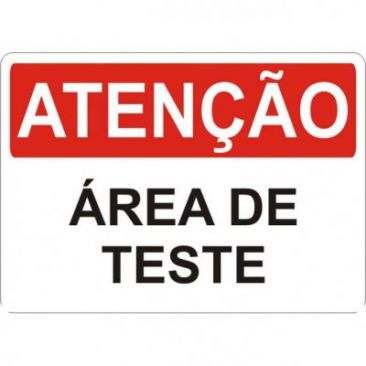
\includegraphics[scale=0.5]{img/teste1.jpeg}
  \caption{Teste 1: vermelho}
  \label{fig:vermelho}
\end{center}
\end{figure}

\begin{figure}[h!]
\begin{center}
   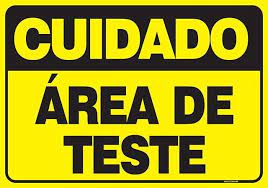
\includegraphics[scale=0.5]{img/teste2.jpeg}
  \caption{Teste 2: amarelo}
  \label{fig:amarelo}
\end{center}
\end{figure}

Para lembrar a \textbf{ordem dos comandos}:

\begin{enumerate}
\itemsep0em
    \item iniciar o ambiente \verb|\begin{figure}|
    \item iniciar a centralização \verb|\begin{center}|
    \item iniciar o comando \verb|includegraphics|
    \begin{enumerate}
        \item definir a especificação da imagem (tamanho...)
    \end{enumerate}
    \item definir uma legenda para tabela \verb|caption|
    \item definir uma etiqueta para ref. cruzada \verb|label|
    \item finalizar a centralização \verb|\end{center}|
    \item finalizar o ambiente \verb|\end{figure}|
\end{enumerate}

O código para as duas figuras acima é:

\begin{codex}{Código de exemplo - Figuras}
%Imagem 1
\begin{figure}[h!]
\begin{center}
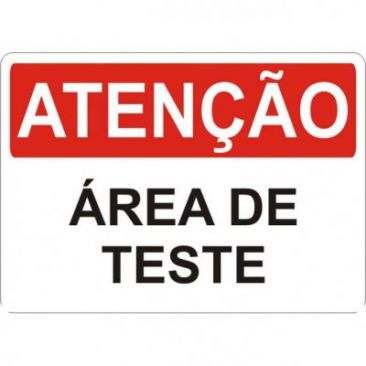
\includegraphics[scale=0.5]{img/teste1.jpeg}
\caption{Teste 1: vermelho}
\label{fig:vermelho}
\end{center}
\end{figure}
%Imagem 2
\begin{figure}[h!]
\begin{center}
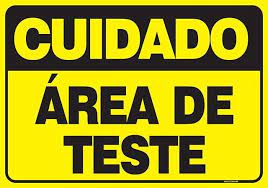
\includegraphics[scale=0.5]{img/teste2.jpeg}
\caption{Teste 2: amarelo}
\label{fig:amarelo}
\end{center}
\end{figure}
\end{codex}
%===================================
\chapter{Ambientes Específicos}

\section{Aspas}

O pacote \verb|textcmds| é responsável pela produção das aspas simples e duplas com certa economia de digitação. Ele está disponível em \url{https://ctan.math.illinois.edu/macros/latex/contrib/amsrefs/textcmds.pdf}.

Observe as aspas nos seguintes exemplos (a fonte maior é intencional...):

\begin{enumerate}
	\item {\LARGE "aspas duplas" produzidas usando "SHIFT" + a tecla abaixo da tecla "Esc".}
	\item {\LARGE 'aspas simples' produzidas usando a tecla abaixo da tecla 'Esc'.}
\end{enumerate}

No primeiro exemplo, as aspas são iguais mas entre as palavras \textit{duplas} e \textit{produzidas} e \textit{SHIFT} e o sinal de ( + ) não há espaços após as aspas. Essa falta de espaço não é um erro de digitação, mas uma questão do \LaTeX. Veja parte do código:

\begin{codex}{aspas duplas}
{\LARGE "aspas duplas" produzidas usando "SHIFT" + a tecla abaixo da tecla "Esc".}
\end{codex}

A digitação está correta, no entanto, o \LaTeX, para produzir aspas precisa da seguinte digitação: \verb|``aspas''|, \textit{i.e.}, dois sinais do acento grave (popularmente conehecido como \textit{crase}), seguido da palavra e só então, dois sinais de aspas simples. Particularmente, considero, no processo de digitação de um texto, esse procedimento muito trabalhoso porque a sequência de teclas é: (i) SHIFT + acento grave 2x + SHIFT + acento grave 2x + palavra ou expressão entre aspas + aspas simples 2x.

Para resolver isso, incluí o pacote \verb|textcmds| que, entre outros aspectos, permite digitar aspas duplas com o comando \verb|\qq{texto}|, em que \textbf{texto} é o que se deseja que fique entre aspas duplas.

Já no segundo exemplo, note que as aspas simples na expressão \textit{aspas simples} e na palavra \textit{Esc} são iguais. Isto é, estão na mesma posição. Novamente, não é erro de digitação. Veja o código:

\begin{codex}{aspas simples}
{\LARGE 'aspas simples' produzidas usando a tecla abaixo da tecla 'Esc'.}
\end{codex}

Novamente, o \LaTeX, para produzir aspas simples precisa da seguinte digitação: \verb|`aspas'|, \textit{i.e.}, SHIFT + sinal de acento grave + palavra ou expressão + aspas simples.

Assim, para aspas simples, o pacote \verb|textcmds| requer que se digite somente \verb|\q{texto}|, em que \textbf{texto} é o que se deseja que fique entre as aspas simples. Veja os exemplos a seguir.

\begin{itemize}
	\itemsep0em
	\item Estas são \qq{aspas duplas}.
	\item Estas são \q{aspas simples}.
	\item Estas são \qq{aspas duplas com \q{aspas simples} ao mesmo tempo}
\end{itemize}

E o código dos exemplos acima é:

\begin{codex}{aspas com o pacote textcmds}
Estas são \qq{aspas duplas}.
Estas são \q{aspas simples}.
Estas são \qq{aspas duplas com \q{aspas simples} ao mesmo tempo}
\end{codex}

\section{Citação longa}

Ver seção \textbf{2.2 Diretas - Maior que 3 linhas}.

\section{Códigos de exemplo}

As caixas de textos para digitação de código podem ser obtidas através do ambiente \textbf{codex}, uma abreviação para \textbf{CÓD}igos de \textbf{EX}emplo.

Essa caixa de texto é iniciada pelo ambiente \verb|\begin{codex}| ... \verb|\end{codex}|. 

\textsc{\textbf{Atenção:}} \LaTeX\ diferencia maiúsculas de minúsculas nos comandos e ambientes.

\noindent\textbf{\textsc{Observe:}}

\begin{codex}{Exemplo de caixa de texto}
Essa é uma caixa de texto de exemplo.
\end{codex}

Note que esse ambiente traz como título a palavra \textbf{Exemplo} seguida de uma numeração automática (\textbf{1.4}) e, em seguida, o texto que você deseja utilizar para nomear o seu exemplo (\textbf{Exemplo de caixa de texto}). Esse último elemento é obrigatório. Além disso, o código a ser digitado já traz a numeração das linhas para facilitar a leitura.

Sempre que você usar esse ambiente, a palavra inicial será sempre \textbf{Exemplo} e a numeração será tanto automática quanto referente à seção primária (normalmente chamada de capítulo) em que você está produzindo. Ou seja, todas as caixas de exemplo utilizadas nessa seção iniciarão com o número \textbf{4}, todos os exemplos utilizados na seção 2, iniciarão com o número 2, e assim por diante. 

Para obter essa caixa de texto, você deve usar o código a seguir: 

\indent\verb|\begin{codex}{Ambiente codex}|\\
\indent\verb|digite o seu código de|\\
\indent\verb|exemplo aqui|\\
\indent\verb|sem se preocupar|\\
\indent\verb|com a numeração das linhas|\\
\indent\verb|\end{codex}|

Onde \verb|\begin{codex}| inicia o ambiente, \verb|{Ambiente codex}| nomeia o exemplo e é obrigatório seu uso, \verb|digite o seu código...| é o código que se deseja demonstrar e \verb|\end{codex}| finaliza o ambiente.

\indent\textsc{Dica:} Caso deseje que haja espaços maiores entre a numeração das linhas e o seu exemplo de código, basta pressionar a barra de espaços (ou tab) quantas vezes quiser.

\begin{codex}{Espaços entre a numeração de linhas e o código}
sem espaço
 com um espaço
  com dois espaços
   com três espaços
    com quatro espaços
     acho que deu para entender...

\end{codex}
%===================================
%Início das Referências
\backmatter{
\renewcommand{\bibname}{Referências}
\bibintoc
\bibliographystyle{abntex2-alf}
\bibliography{references}
%Se o trabalho não tiver apêndices ou anexos
%excluir ou comentar a linha abaixo.
%para insruções, ver arquivo postext.tex
%Anexos
\thispagestyle{empty}
\part*{Anexos} % Se quiser uma página antes dos apêndices
\addcontentsline{toc}{part}{Anexos}

\chapter*{Anexo A -- Um anexo}
\addcontentsline{toc}{chapter}{Anexo A -- Um anexo}


%Apendices
\thispagestyle{empty}
\part*{Apêndices} % se quiser uma página antes dos apêndices
\addcontentsline{toc}{part}{Apêndices}

\chapter*{Apêndice A -- Um apêndice}
\addcontentsline{toc}{chapter}{Apêndice A -- Um apêndice}


%Última folha em branco
\newpage
\thispagestyle{empty}
}

%===================================
%Fim das Referências
\end{document}